\chapter{Tag Clouds}
\label{sec:semannot}

\begin{summary}
This chapter presents an overview of tagclouds used as a method for representing text content.
\end{summary}

Tag Clouds are popular applications used for vaious purposes: as a navigation mechanism, as indicators of activity within social media experiences, for visualization in texts and textual data, for annotation of documents~\ref{fig:tagcloud}. The importance or weight of words in the tag cloud are shown with size of font and/or color. The tag clouds are hyperlinks leading to a collection of items associated with the tag.\\
A version of tag cloud is called text cloud. It is used as a visual display that conveys the broad themes that emerge from textual analysis.  
There are three types of tag clouds depeding on their purpose and use. The first type contains a tag represeting the frequency of each term. The second type is a global tag cloud whose tags has frequencies aggreggated over all items and users. The third type of tag cloud contains categories, and its tags' size indicates the number of subcategories.\\
%TODO
%generate a tag cloud based on the contents in docmachine!!!!!!! replace the figure
%
% Opencloud
%
\begin{figure}[htbp]
	\centering
	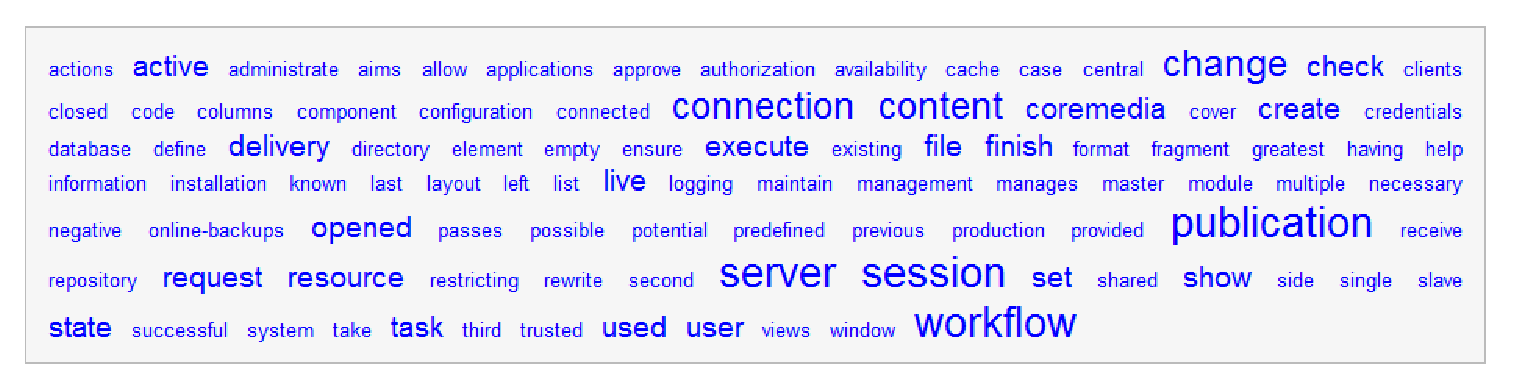
\includegraphics[width=\ScaleIfNeeded]{img/tagcloud} 
 % or [scale=0.5]
	\caption{Tag Cloud}
	\label{fig:tagcloud}
\end{figure}

\section{1}
\label{sec:semannot:1}
Related work 
SenseBot Search Results Summarizer is a plugin for Mozilla Firefox browser that generates a tag cloud of the main concepts returned as search results from Google.

LinkSensor
SenseBotSummarizer
All three are based on SenseBot - a semantic search engine.
Made available from Semantic Firefox Extensions \footnote{\url{http://www.semanticengines.com/plugins.htm}}\\

\section{Brainstorming}
What is a tag cloud? Graphical representation of a collection of tags. Tag clouds visualize word frequency in a given text.\\

Tag clouds may be used as a topic summary.\\

There are three main types of tag cloud applications used in social software.\\
\begin{enumerate}
\item frequency of items / tags
\item number of items to which a tag has been applied
\item tags are categorization method for content items 
\end{enumerate}
The following tag clouds were evaluated in order to select the solution that is most applicable for Tag Cloud Summarizer project.\\
\begin{itemize}
\item TagsTreeMaps\footnote{\url{http://tagstreemaps.sourceforge.net/TagsTreeMaps.html}}
\item OpenCloud\footnote{\url{http://opencloud.sourceforge.net/}}
\end{itemize}
